\chapter{Sistemi retroazionati}

\begin{figure}[h!]
  \centering
  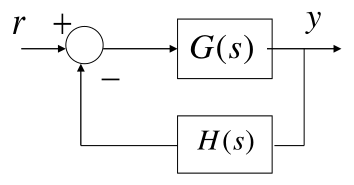
\includegraphics[scale=0.3]{./images/schema_blocchi.png}
\end{figure}

La funzione di trasferimento \`e:

\begin{align}
  f.d.t. = \frac{Y(s)}{X(s)} = \frac{G(s)}{1 + G(s)H(s)}
\end{align}


% \section{Analisi a regime dei sistemi in retroazione}
% \subsection{Gradino}
%
% \begin{align}
%   e_r = \lim_{s \to 0} sE(s) = \frac{r_0}{1 + K}
% \end{align}



